\chapter{Física de Altas Energias e o Projeto LHC}
\label{chap:lhc}

Como se sabe, tudo no universo é formado por partículas elementares, governadas por poucas forças fundamentais. Algumas destas partículas são estáveis e formam a matéria conhecida. Já as partículas instáveis duram apenas frações de segundo antes de decaírem em partículas estáveis. Ambas as classes de partículas coexistiram por um breve momento após o Big Bang. Desde então, para fazer com que estas partículas instáveis surjam novamente, uma maneira é colidir partículas com enorme quantidade de energia, de forma a recriar, em laboratório, o ambiente presente no momento do Big Bang \cite{bib:cern}.

Para recriar este ambiente, os físicos utilizam colisionadores de partículas, os quais são compostos por dutos onde um feixe de partículas é acelerado à velocidades bastante elevadas, de forma a aumentar consideravelmente a energia destas. Quando a energia chega a um ponto suficientemente elevado, o feixe é posto para colidir com um outro grupo de partículas (que podem estar tanto paradas, como sendo aceleradas em sentido contrário), recriando, no momento da colisão, o ambiente propício para a formação de partículas instáveis. Com isto, pretende-se estudar a estrutura da matéria. Como as partículas são aceleradas utilizando-se poderosos campos magnéticos, as mesmas precisam possuir carga. Assim sendo, normalmente são utilizados prótons ou elétrons no feixe a ser acelerado.

\section{O Modelo Padrão}

As teorias e descobertas de milhares de físicos durante o século passado criaram uma notável imagem da estrutura fundamental da matéria: o Modelo Padrão de Partículas e Forças \cite{bib:hep}.

O Modelo Padrão requer 12 partículas elementares e 4 partículas transportadoras de força para resumir tudo o que é atualmente conhecido sobre os mais fundamentais constituintes da matéria e suas interações. O Modelo Padrão é, por hora, uma teoria física bem testada, usada para explicar e predizer exatamente uma vasta variedade de fenômenos. Entretanto, os físicos sabem que existem teorias ainda não confirmadas, de tal forma que diferentes experimentos ainda devem ser realizados para confirmá-las.


\subsection{Partículas Materiais}

Existem duas famílias de partículas materiais: os quarks e os leptons, ambos sem estrutura interna:

\begin{itemize}

\item \textbf{Quarks:} são 6, freqüentemente agrupados em 3 pares, devido à suas propriedades de massa e carga:
    \begin{itemize}
        \item up/down
        \item charm/strange
        \item top/bottom
    \end{itemize}

\item \textbf{Leptons:} são 6, agrupados em duas categorias, cada uma contendo 3 tipos:

    \begin{itemize}
        \item \textbf{Com carga e massa:} elétron ($e^-$), múon ($\mu$) e tau
        ($\tau$).

        \item \textbf{Neutras e com massa reduzida:} elétron-neutrino ($V_e$),
múon-neutrino ($V_\mu$) e tau-neutrino ($V_\tau$).

        \end{itemize}

        Como os nomes desta categoria sugerem, estas 6 partículas também podem ser agrupadas em três pares ($\mu^-/V_\mu$, por exemplo.)

\end{itemize}

A matéria estável do universo é formada apenas pelos pares mais leves $e^-/V_e$ e up/down, formando a chamada primeira geração da matéria. Entretanto, processos de alta energia produzem uma grande variedade de partículas de vida curta, que requerem a existência de pares mais pesados. Assim, tem-se os pares $\mu/V_\mu$ e
charm/strange, que formam a segunda geração, enquanto que os pares $\tau/V_\tau$ e top/bottom formam a terceira geração da matéria.

\subsection{Partículas Transportadoras de Força}

O Modelo Padrão considera 3 tipos de forças atuando entre partículas: força forte, fraca e eletromagnética (a gravidade ainda não é parte da estrutura).

As forças são comunicadas entre as partículas através da troca de partículas transportadoras de força, chamadas de bósons, que carregam uma quantidade discreta de energia de uma partícula a outra. Cada força tem seus próprios bósons característicos: o glúon (força forte), o fóton (força eletromagnética) e os bósons
$W$ e $Z$ (força fraca).

O Modelo Padrão é, atualmente, a melhor descrição que se tem do mundo das partículas. Entretanto, existem importantes teorias que o Modelo Padrão ainda não pode comprovar experimentalmente. Entre estas, temos: \emph{qual a origem da massa das partículas?}

Partículas possuem uma vasta variedade de massas. Fótons e glúons são completamente desprovidos de massa, enquanto que as partículas $W$ e $Z$ pesam, cada uma, tanto quanto 80 a 90 prótons. A partícula mais pesada descoberta até agora, o quark top, é duas vezes mais pesado que os bósons $W$ e $Z$, pesando aproximadamente o mesmo
que um núcleo de ouro. Entretanto, o porquê da existência desta larga faixa para as massas ainda é um mistério. De fato, a maneira como as partículas adquirem massa ainda não é devidamente compreendida.

No Modelo Padrão, sugere-se que as partículas ganham uma massa através do mecanismo de Higgs. De acordo com esta teoria, tanto as partículas de matéria como as transportadoras de forças interagem com uma nova partícula, o \textbf{Bóson de Higgs}. A força desta interação é o que dá lugar ao que se chama de massa. Ou seja:
quanto maior a interação, maior a massa.

Experimentos ainda precisam mostrar se esta teoria é correta. A busca pelo bóson de Higgs já começou no colisionador LEP, no CERN \cite{bib:cern}, e em outros experimentos. E esta busca continuará com o próximo colisionador, que está em construção no CERN, o LHC.




\section{O Projeto LHC (\emph{Large Hadron Collider})}


O LHC \cite{bib:lhc} é um novo acelerador que entrará em operação em 2007. Com seus magnetos poderosos, e possuindo incríveis 27 km de circunferência, ele será capaz de atingir níveis de energia nunca antes alcançados, devendo colidir pacotes com um número elevado de prótons com 14 Tev no centro de massa. Com esta energia, espera-se tornar possível a comprovação experimental da existência do bóson de Higgs.


Os prótons são acelerados em tubos a vácuo em túneis subterrâneos. Eles são mantidos em órbitas aproximadamente circulares por fortes campos magnéticos produzidos por imãs supercondutores. Entretanto, quanto maior a energia, maior a órbita das partículas, e, conseqüentemente, maior o túnel. Desta maneira, o LHC (vide Figura \ref{fig:vista_aerea_lhc}) constitui o maior acelerador de partículas do mundo.

\begin{figure}
\begin{center}
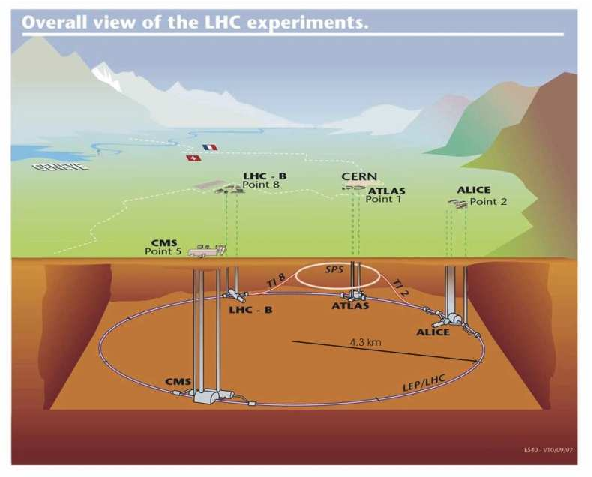
\includegraphics[height = 6.5cm]{top_view_lhc}
\caption[Vista aérea do LHC.]{Vista aérea do LHC (extraído de \cite{bib:site_lhc}).}
\label{fig:vista_aerea_lhc}
\end{center}
\end{figure}

Como os feixes de prótons trafegam por tubos separados, para colidi-los é feito o seguinte: em pontos específicos do acelerador, chamados de ``pontos de colisão'', não existem campos magnéticos, de forma que, nestas regiões, os feixes percorrem uma trajetória retilínea. Desta maneira, os dois feixes podem ser reunidos em um ambiente a vácuo e postos, finalmente, em rota de colisão.

Os prótons são inseridos no acelerador em rajadas de uns poucos centímetros de comprimento e alguns micrômetros de raio. A distância entre uma rajada e outra é de 7,5 metros. Uma vez que a luz demora 25 nanosegundos para percorrer 7,5 metros, e os prótons estão praticamente se movendo à velocidade da luz, conclue-se que as rajadas irão cruzar-se (e os prótons colidirem) com uma freqüência de 40 MHz. Entretanto, o número de colisões entre prótons depende da quantidade de prótons em cada rajada, o tamanho dos mesmos e do desenho do acelerador. Para uma alta taxa de
colisões, deve-se ter rajadas de curto comprimento, muitos prótons por rajada e muitas rajadas por unidade de tempo. Estas propriedades, que dependem do projeto do acelerador, podem ser combinadas em um único parâmetro: \textbf{luminosidade}.

A luminosidade é definida como a constante de proporcionalidade entre a taxa de colisões entre prótons e a área do próton. Em física experimental de partículas, atingir níveis elevados de luminosidade é tão importante quanto atingir níveis elevados de energia. Isto ocorre porque nem todas as colisões produzem os mesmos efeitos, e os tipos de colisões que geram eventos de interesses são extremamente raros. Por isso, são necessárias muitas colisões distintas (ou seja, alta luminosidade) para que se aumente a probabilidade de observação de eventos de interesse. No LHC, espera-se, com a luminosidade de operação ($1 \times 10^{34}$ cm$^{-2}$ s$^{-1}$ \cite{bib:tdaq_tdr}), atingir um total de um bilhão de colisões por segundo, sendo que deste valor, apenas um número entre 10 e 100 colisões poderão vir a ser de potencial interesse científico. No caso do bóson de Higgs, dada a sua raridade, esta taxa pode cair para um valor tão baixo que serão necessárias horas, e até mesmo dias, para que um único decaimento deste tipo possa vir a ocorrer.

Entretanto, para que seja possível aos físicos realizar as análises necessárias nos eventos gerados durante a colisão, sistemas de detecção devem ser posicionados em torno dos pontos de colisão para realizar a captura dos eventos gerados, e convertê-los em informação interpretável para os físicos. Visando este fim, o LHC possui diversos detectores:

\begin{itemize}

\item \textbf{ATLAS (\emph{A Toroidal LHC Apparatus})} $\rightarrow$ Este experimento, composto por vários detectores, será capaz de, entre outras coisas, provar experimentalmente a existência do bóson de Higgs. Detalhes deste experimento serão vistos na seção \ref{SEC:ATLAS}.

\item \textbf{CMS (\emph{Compact Muon Solenoid})} $\rightarrow$ A maioria dos detectores em física de partículas estão posicionados em torno de dispositivos magnéticos, de forma a tornar possível medir o momento de partículas carregadas. Este experimento contará com um solenóide supercondutor capaz de gerar um campo magnético de 4T (cem mil vezes maior do que o campo magnético da Terra), permitindo que dispositivos de detecção de traços e calorimetria sejam inseridos dentro das espiras do solenóide gerador do campo magnético, resultando em um poderoso detector de uso geral, composto inclusive, por detectores de múons \cite{bib:cms}.

\item \textbf{LHCb (\emph{A High Energy Physics Experiment Studying CP Violation})} $\rightarrow$ Este experimento visa estudar a violação CP\footnote{No mundo atômico, cada elemento possui a sua imagem ``espelhada'' (neutrinos e anti-neutrinos, por exemplo), entretanto, a anti-matéria nem sempre se comporta como uma imagem espelhada da matéria, de tal forma que a este fenômeno dá-se o nome de violação CP.}. Com o detector sendo desenvolvido neste experimento, os físicos serão capazes de detectar minúsculas diferenças entre matéria e anti-matéria \cite{bib:lhcb}.

\item \textbf{ALICE (\emph{A Large Ion Collider Experiment})} $\rightarrow$ O projeto ALICE consiste em um detector dedicado de íons pesados que explorará as interações entre núcleos atômicos ocorridas à energias elevadas, como as fornecidas pelo LHC. O objetivo é estudar a física de matérias fortemente interativas à densidades de energia elevadíssimas, onde se espera a formação de uma nova fase da matéria: o plasma quark-glúon \cite{bib:alice}.

\item \textbf{TOTEM (\emph{Total Cross Section, Elastic Scattering
and Diffraction Dissociation})} $\rightarrow$ Este experimento é dedicado a medir a seção transversal total, dispersão elástica e processos difrativos no LHC. Com isso, espera-se fornecer uma calibração exata da luminosidade do LHC \cite{bib:totem}.

\end{itemize}



\section{O Detector ATLAS (\emph{A Toroidal LHC Apparatus})}
\label{SEC:ATLAS}

\begin{figure}
\begin{center}
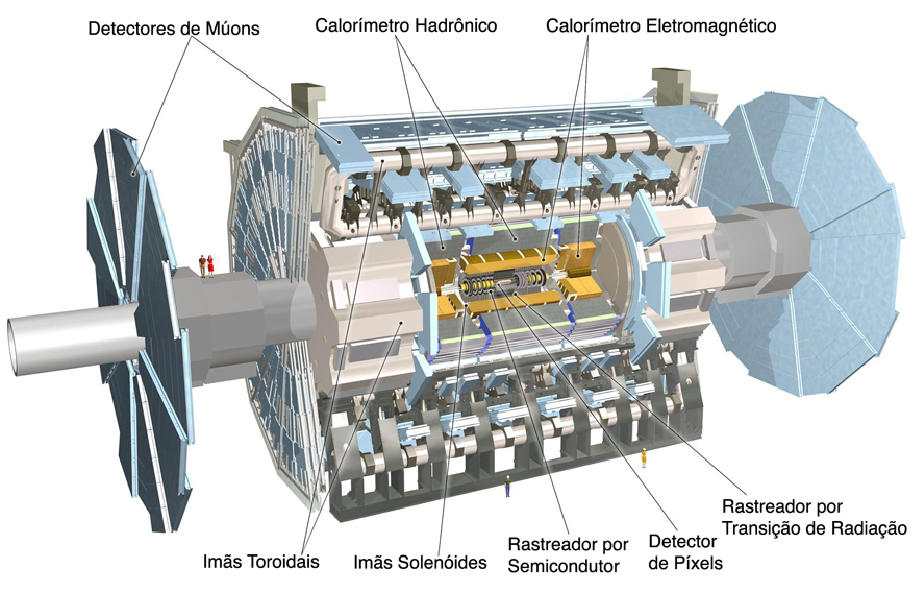
\includegraphics[height = 7cm]{atlas_detector}
\caption[Diagrama ilustrativo do detector ATLAS.]{Diagrama ilustrativo do detector ATLAS (extraído de \cite{bib:atlas}).}
\label{FIG:DETECTOR_ATLAS}
\end{center}
\end{figure}

Quando prótons colidem, alguns dos eventos gerados podem trazer informações relevantes ao experimento, enquanto que muitas outras colisões ordinárias (que não trazem nenhuma informação nova, e por isso, são comumente tratadas como ruído de fundo da experiência) são adquiridas. Assim, uma das principais necessidades de experimentos realizados com aceleradores de partículas é a separação dos eventos de interesse dos eventos de física ordinária. A diferenciação entre eventos é baseada nos produtos observados em cada colisão: energia, direção de movimento, etc. Para se identificar os eventos de interesse, torna-se necessário um poderoso detector que fornecerá informação detalhada sobre os produtos obtidos através das colisões realizadas no LHC. Este é o caso do detector ATLAS \cite{bib:site_atlas}. O projeto deste detector é o maior esforço colaborativo jamais visto na física, envolvendo 1800 cientistas de mais de 150 universidades em 34
países.

Observa-se, na Figura \ref{FIG:DETECTOR_ATLAS}, um diagrama ilustrativo do detector ATLAS, dando idéia de suas dimensões. Este detector está dividido em módulos distintos, conforme se pode analisar observando-se a seção transversal do mesmo, apresentada na Figura \ref{FIG:SECAO_TRANSVERSAL_ATLAS}, onde cada número indica um módulo específico, a saber:

\begin{figure}
\begin{center}
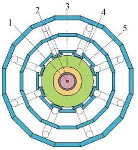
\includegraphics[height = 5.5cm]{atlas_detector_crossview}
\caption[Seção transversal do detector ATLAS.]{Seção transversal do detector ATLAS (extraído de \cite{bib:site_atlas}).}
\label{FIG:SECAO_TRANSVERSAL_ATLAS}
\end{center}
\end{figure}

\begin{enumerate}

\item \textbf{Tubo do Feixe:} o tubo do feixe passa através do centro do detector e carrega o feixe de prótons. Feixes viajando em sentido contrário através deste tubo são postos para colidir no meio do detector.

\item \textbf{Detector de Traços:} a região interna do detector está repleta de sensores altamente segmentados feitos de tiras de silício, de forma que a trajetória de partículas carregadas possa ser precisamente determinada. A trajetória de uma partícula carregada é curva, se a mesma estiver sob a influência de um campo magnético. O raio da curvatura e a direção da deflexão indicam, respectivamente, o momento e a carga da partícula.

\item \textbf{Calorímetro Eletromagnético:} este calorímetro consiste em finas pastilhas de chumbo (1,5 mm de espessura) separadas por sensores. Quando fótons ou elétrons de alta energia atravessam o chumbo (ou outro material de número atômico elevado), eles produzem um chuveiro eletromagnético\footnote{Um chuveiro eletromagnético ocorre quando um elétron (ou pósitron) é deflexionado pelo campo elétrico dos átomos, fazendo com que estes emitam fótons. Os fótons, por sua vez, geram elétrons (ou pósitrons), que por sua vez, geram mais fótons, e assim sucessivamente.}. O que acontece é que a energia inicial destas partículas é convertida em um grande número de elétrons e pósitrons de mais baixa energia, mas ainda em alta velocidade. O número final de elétrons / pósitrons é proporcional à energia da partícula incidente. 

As pastilhas de chumbo estão imersas em um tanque de argônio líquido. As reentrâncias (aproximadamente 4 mm), preenchidas com argônio líquido entre as pastilhas, estão sujeitas a um forte campo elétrico. Quando um chuveiro de elétrons, produzido dentro do chumbo, chega ao argônio, ele gera um rastro de pares elétrons-íons ao longo do seu caminho \cite{bib:knoll_radiation_detection}. O campo elétrico, então, faz com que os elétrons migrem para o lado positivo (muito mais rapidamente do que os íons migram para o lado negativo), gerando uma corrente elétrica em um circuito externo conectado ao calorímetro. Quanto maior a energia incidente, maior o número de chuveiros de elétrons e, conseqüentemente, maior a corrente gerada.

Este calorímetro está dividido em quatro camadas sobrepostas, com espessuras específicas, onde a terceira camada é a mais espessa. Além disso, cada camada possui granularidade específica, o que ajuda a determinar alguns aspectos dos objetos que interagem com este detector \cite{bib:msc_rabello}. Por fim, visando a redução de custos, a granularidade varia dentro de uma mesma camada, sendo menor (menor resolução) nas bordas do detector, regiões onde o aparecimento de eventos de interesse serão mais raros.

As conexões elétricas com o calorímetro são feitas, de fato, a finos membros metálicos imersos em argônio líquido (eletrodos). Estes eletrodos são subdivididos em pequenas regiões retangulares. Tais regiões, a várias profundidades, são agrupadas e unidas para formar camadas, de tal forma que, quando uma partícula atinge este calorímetro, tem-se a informação da energia depositada através de várias camadas, aumentando a resolução da detecção, uma vez que se adiciona mais uma dimensão de observação da interação de partículas com este calorímetro.

\item \textbf{Calorímetro Hadrônico:} este dispositivo mede a energia dos hadrons que o atingem, incluindo prótons, nêutrons, píons e káons (elétrons e fótons foram absorvidos na seção eletromagnética). O calorímetro hadrônico consiste em absorvedores metálicos separados por telhas de material cintilante. A interação de hadrons de alta energia com os absorvedores transformam a energia incidente em um chuveiro hadrônico, constituído por vários prótons e nêutrons de baixa energia, e outros hadrons. Este chuveiro, quando atravessa o material cintilante, faz com que este emita luz, em quantidade proporcional à energia incidente. Entretanto, uma vez que os hadrons podem iniciar seus chuveiros no calorímetro eletromagnético, os sinais obtido pelos dois calorímetros precisam ser somados para se obter a energia hadrônica total. Tal como o calorímetro eletromagnético, o calorímetro hadrônico também está dividido em camadas, possuindo, neste caso, três camadas sobrepostas, de forma a acrescentar mais uma dimensão de observação da deposição de energia.

A energia total emanada do ponto de colisão é menos intensa para grandes angulações (próximo a 90 graus), e mais intensa a ângulos menores em relação ao feixe. Devido ao fato que as telhas cintilantes podem se danificar se expostas à radiação, a calorimetria hadrônica, para ângulos entre 5 e 25 graus, é fornecida por um dispositivo de argônio muito similar ao utilizado no calorímetro eletromagnético. As principais diferenças são que as pastilhas de chumbo são substituídas por pastilhas de cobre (com espessura de 2,5 cm), que são mais apropriadas para o chuveiro hadrônico, e as reentrâncias entre as pastilhas distam 8 mm uma das outras.

\begin{figure}
\begin{center}
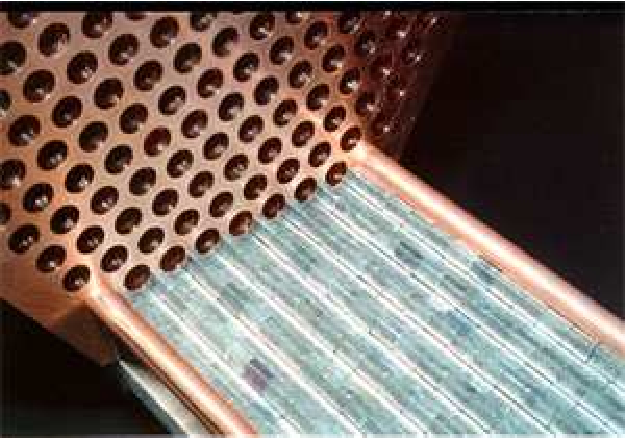
\includegraphics[height = 5cm]{hadron_forward}
\caption[Ilustração das barras metálicas sendo inseridas nos tubos da calorímetro de argônio líquido do calorímetro hadrônico.]{Ilustração das barras metálicas sendo inseridas nos tubos da calorímetro de argônio líquido do calorímetro hadrônico (extraído de \cite{bib:site_atlas}).}
\label{FIG:BARRAS_CALORIMETRO_HADRONICO}
\end{center}
\end{figure}

Para permitir a cobertura angular total, é necessário estender o calorímetro para que este detecte jatos a ângulos tão pequenos quanto 1 grau relativo aos feixes. Devido ao ambiente extremamente radioativo na região angular entre um e cinco graus, a calorimetria precisa ser desenvolvida com cuidados especiais. Nesta região, o calorímetro de argônio líquido tem suas pastilhas metálicas substituídas por uma matriz metálica que contém tubos ocos embutidos, de diâmetro interno de 5 mm. Barras metálicas de 4,5 mm são posicionadas dentro destes tubos (vide Figura \ref{FIG:BARRAS_CALORIMETRO_HADRONICO}), e o argônio líquido preenche o pequeno espaço existente entre as barras e os tubos que as contém. Algumas centenas de volts entre uma barra e um tubo produzem o campo elétrico necessário para fazer os elétrons migrarem dentro do argônio líquido, após a ionização gerada pelo chuveiro hadrônico.


\item \textbf{Detector de Múons:} múons interagem com qualquer partícula carregada. Entretanto, como são cerca de 200 vezes mais pesados do que elétrons, estas partículas são muito menos afetadas pelo campo elétrico dos átomos que estejam no caminho desta partícula. Desta forma, múons não geram chuveiros eletromagnéticos, dissipando pouca energia, e somente através da ionização de átomos que estejam em seu caminho. Assim, qualquer partícula energética que chegue a este detector é classificada como múon ou neutrino, visto que as demais partículas foram totalmente absorvidas pelos calorímetros. Entretanto, neutrinos também não interagem com este detector, escapando do mesmo. A presença de neutrinos, desta forma, só pode ser inferida pela energia que sobra do processo.

\end{enumerate}

Cada módulo observará um conjunto específico de propriedades das partículas. Estes módulos são empilhados de tal forma que as partículas possam percorrem todas as camadas seqüencialmente. Uma partícula não se tornará visível até que interaja com uma ou mais camadas do detector, ou que se decomponha em partículas que o façam. Pode-se visualizar, na Figura \ref{FIG:INTERACAO_PARTICULAS_ATLAS}, um exemplo de interação de diversas partículas com as diferentes camadas (módulos) do detector. Como se pode observar, partículas carregadas, como prótons e elétrons, são detectadas tanto na câmara de traços, bem como no calorímetro eletromagnético. Partículas neutras, como nêutrons e fótons, não são detectadas na câmara de traços, só sendo observadas quando interagem com outras camadas do detector. Fótons são detectados somente no calorímetro eletromagnético, enquanto que nêutrons são detectados somente no calorímetro hadrônico. Ou seja, cada partícula deixa a sua própria assinatura, ao interagir com um ou mais módulos do detector. 

\begin{figure}
\begin{center}
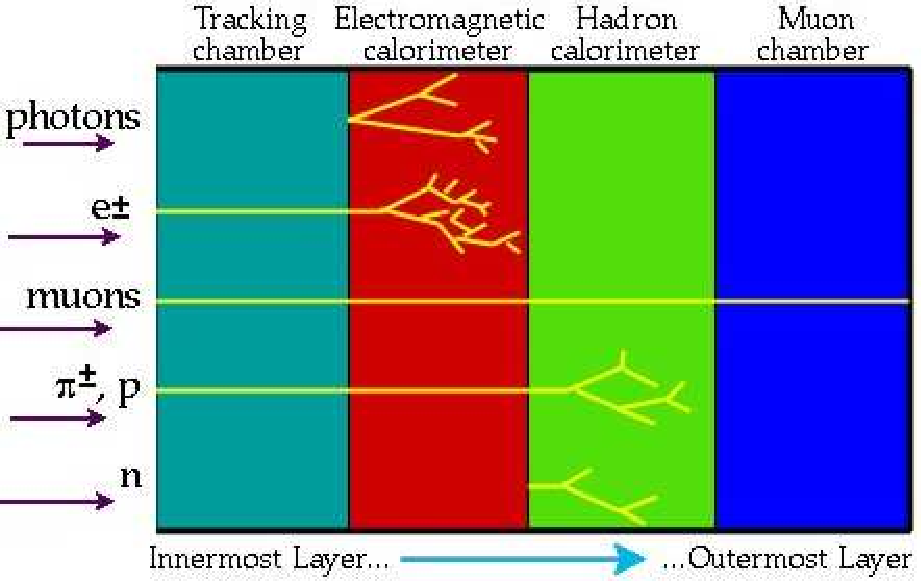
\includegraphics[height = 5.5cm]{decay_chart}
\caption[Interação de diferentes partículas com os diversos módulos do detector ATLAS.]{Interação de diferentes partículas com os diversos módulos do detector ATLAS (extraído de \cite{bib:site_atlas}).}
\label{FIG:INTERACAO_PARTICULAS_ATLAS}
\end{center}
\end{figure}


Espera-se, para este detector, que cada evento gere aproximadamente 1 Mbyte de informação, mas como a taxa de geração de eventos é de 40 MHz, o fluxo de dados será da ordem de 40 TBytes por segundo, o que é um valor impossível de ser armazenado para processamento \emph{offline}, uma vez que o experimento será executado por vários dias. Além disso, pouquíssimos eventos serão de real interesse para o experimento, de tal maneira que um sistema de filtragem \emph{online} deve ser desenvolvido para selecionar somente os eventos de potencial interesse para o projeto, descartando os que não apresentem informação nova, reduzindo desta maneira, o fluxo de informação a ser armazenada para posterior análise.


\huge
***FALAR O QUE SAO ELETRONS E JATOS (EXPLICAR CIENTIFICAMENTE PQ ELES SAO IMPORTANTES)***
\normalsize
